\documentclass[./main.tex]{subfiles}
\begin{document}

% Slide # 3
\begin{frame}[t, label=slide03]
        % Title
        \frametitle{Critical transitions and warning signs}

        % Body
        \footnotesize
        \begin{definition}
                Early warning signals (EWSs) are simple properties that \textbf{change in characteristic ways} prior to a critical transition.
        \end{definition}

        \begin{columns}[T]

                \column{0.5\textwidth}

                \vspace{-0.25cm}
                \uncover<2->{
                        \begin{figure}[H]
                                \centering 
                                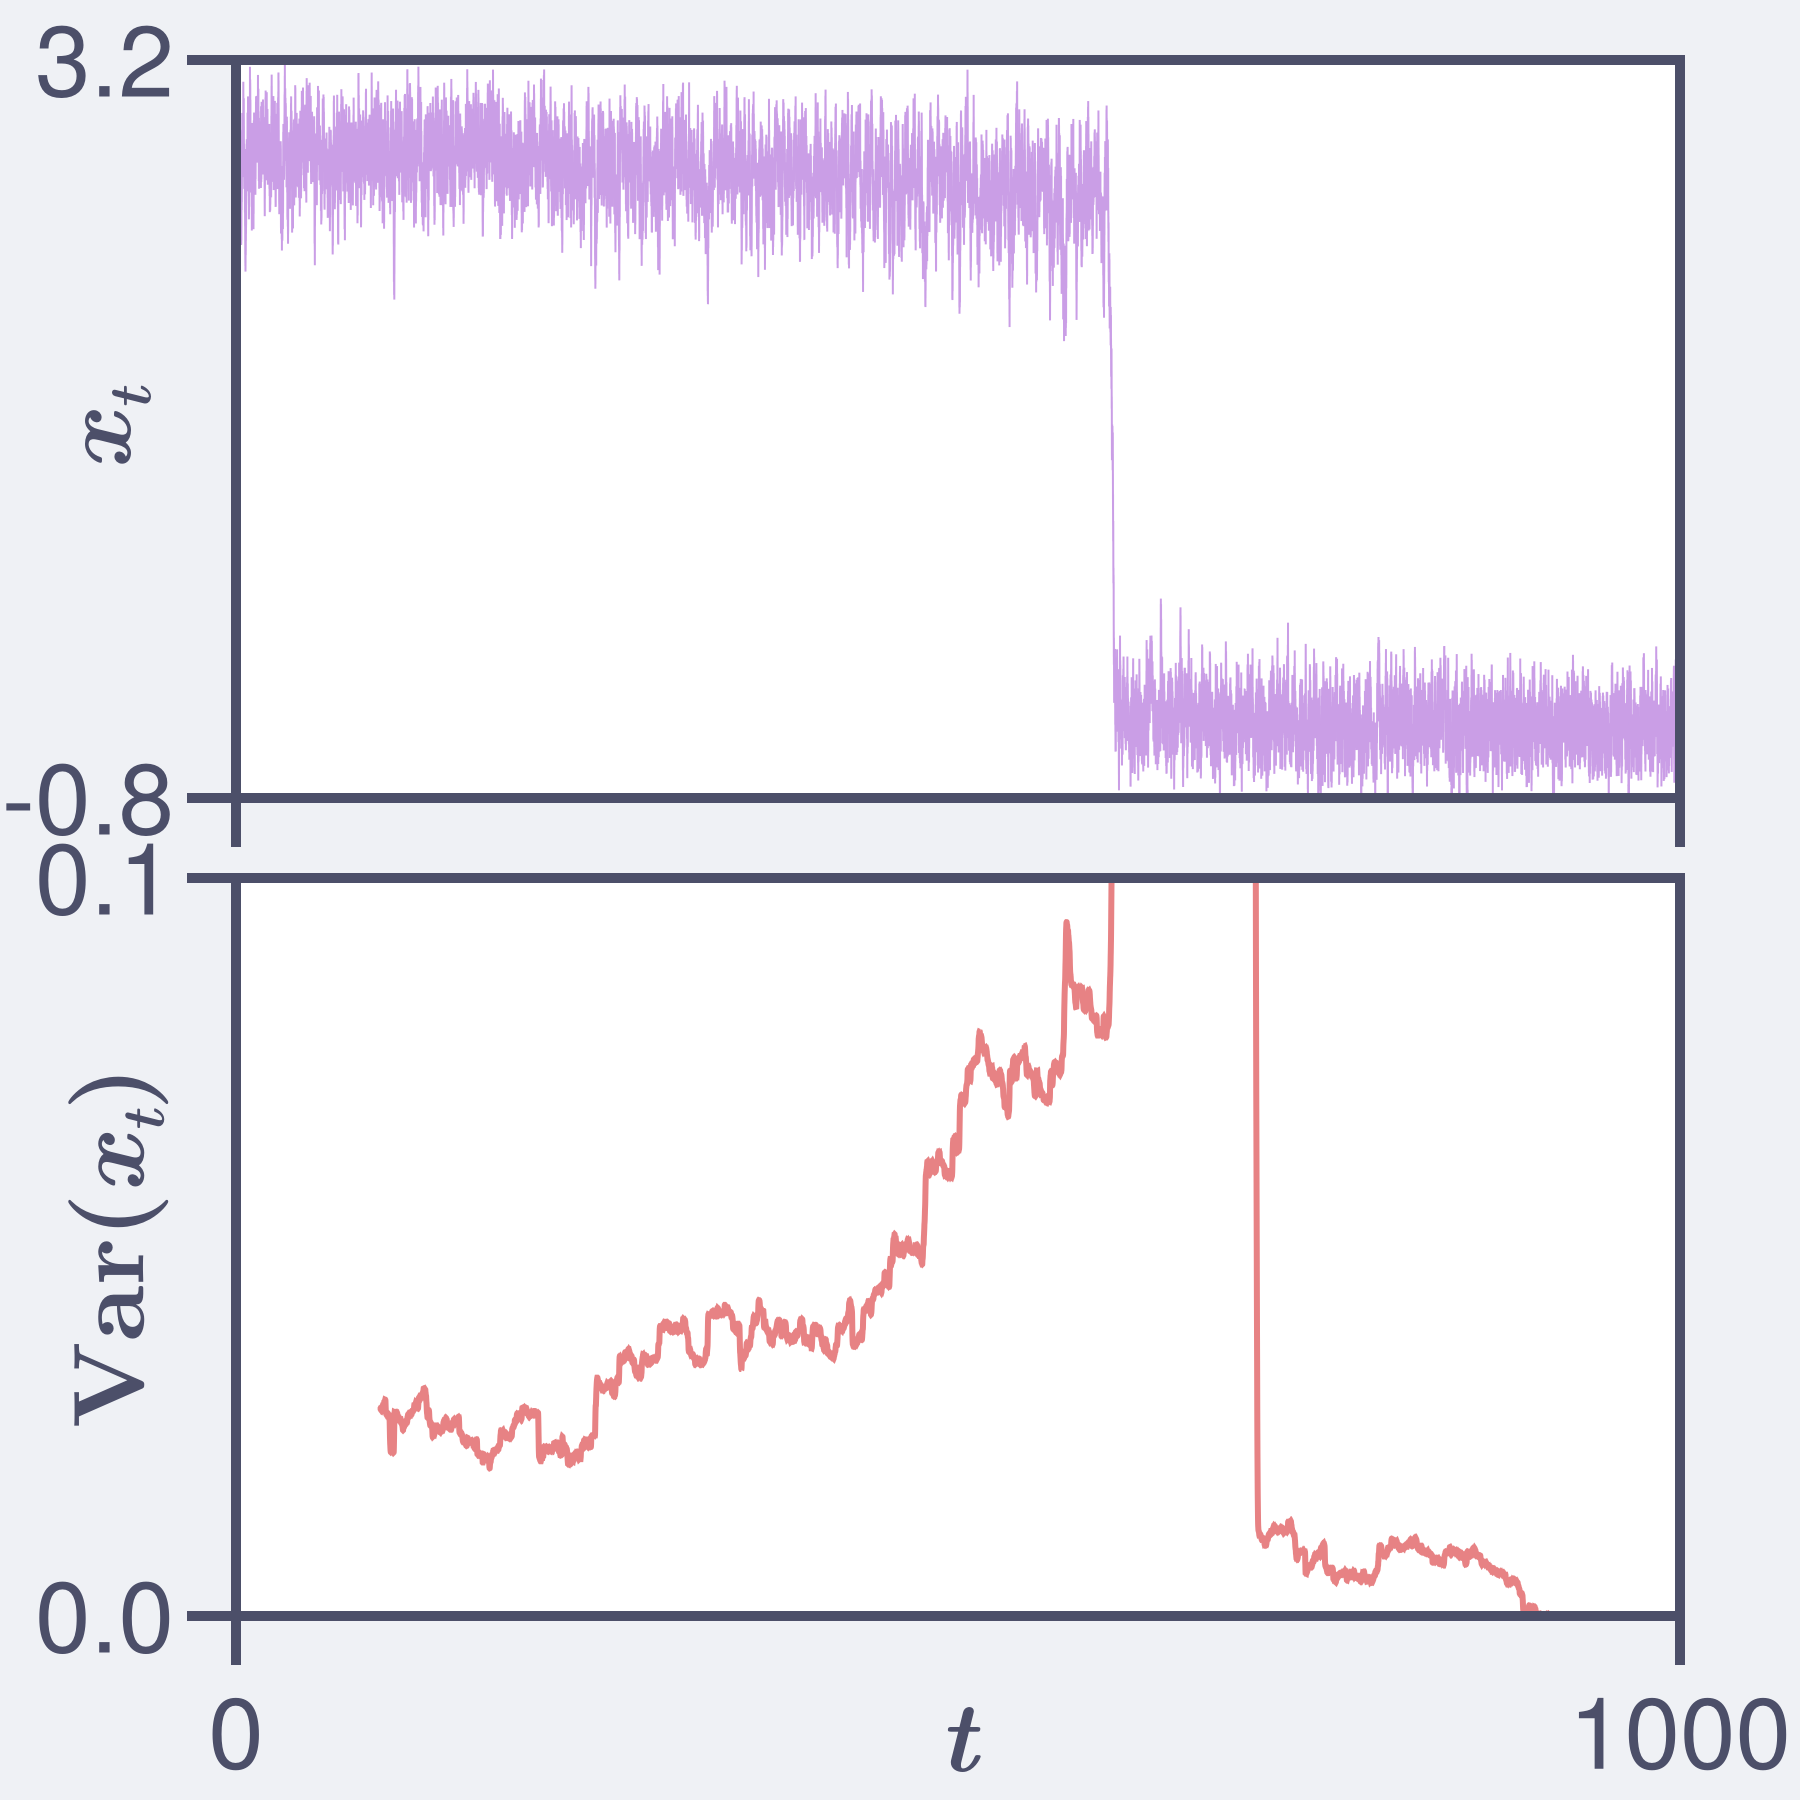
\includegraphics[keepaspectratio, width=\textwidth]{./figures/slide_03.png}
                        \end{figure}
                }

                \hfill
                
                \column{0.5\textwidth}

                \vspace{0.5cm}
                \uncover<3->{
                        The escape rate can be used as an EWS.

                        \bigskip

                        Can we estimate it from \textbf{timeseries data alone}?
                }

                \vspace{0.5cm}
                \uncover<4->{
                        \textbf{Algorithm}:
                        \begin{enumerate}
                             \item detrend the timeseries;
                             \item assemble its histogram;
                             \item fit an optimal density;
                             \item reconstruct the potential;
                             \item compute $\tau_{\text{esc}}$.
                        \end{enumerate}
                }

        \end{columns}
\end{frame}

\end{document}
